% Options for packages loaded elsewhere
\PassOptionsToPackage{unicode}{hyperref}
\PassOptionsToPackage{hyphens}{url}
\PassOptionsToPackage{dvipsnames,svgnames,x11names}{xcolor}
%
\documentclass[
  letterpaper,
  DIV=11,
  numbers=noendperiod]{scrartcl}

\usepackage{amsmath,amssymb}
\usepackage{iftex}
\ifPDFTeX
  \usepackage[T1]{fontenc}
  \usepackage[utf8]{inputenc}
  \usepackage{textcomp} % provide euro and other symbols
\else % if luatex or xetex
  \usepackage{unicode-math}
  \defaultfontfeatures{Scale=MatchLowercase}
  \defaultfontfeatures[\rmfamily]{Ligatures=TeX,Scale=1}
\fi
\usepackage{lmodern}
\ifPDFTeX\else  
    % xetex/luatex font selection
\fi
% Use upquote if available, for straight quotes in verbatim environments
\IfFileExists{upquote.sty}{\usepackage{upquote}}{}
\IfFileExists{microtype.sty}{% use microtype if available
  \usepackage[]{microtype}
  \UseMicrotypeSet[protrusion]{basicmath} % disable protrusion for tt fonts
}{}
\makeatletter
\@ifundefined{KOMAClassName}{% if non-KOMA class
  \IfFileExists{parskip.sty}{%
    \usepackage{parskip}
  }{% else
    \setlength{\parindent}{0pt}
    \setlength{\parskip}{6pt plus 2pt minus 1pt}}
}{% if KOMA class
  \KOMAoptions{parskip=half}}
\makeatother
\usepackage{xcolor}
\setlength{\emergencystretch}{3em} % prevent overfull lines
\setcounter{secnumdepth}{5}
% Make \paragraph and \subparagraph free-standing
\makeatletter
\ifx\paragraph\undefined\else
  \let\oldparagraph\paragraph
  \renewcommand{\paragraph}{
    \@ifstar
      \xxxParagraphStar
      \xxxParagraphNoStar
  }
  \newcommand{\xxxParagraphStar}[1]{\oldparagraph*{#1}\mbox{}}
  \newcommand{\xxxParagraphNoStar}[1]{\oldparagraph{#1}\mbox{}}
\fi
\ifx\subparagraph\undefined\else
  \let\oldsubparagraph\subparagraph
  \renewcommand{\subparagraph}{
    \@ifstar
      \xxxSubParagraphStar
      \xxxSubParagraphNoStar
  }
  \newcommand{\xxxSubParagraphStar}[1]{\oldsubparagraph*{#1}\mbox{}}
  \newcommand{\xxxSubParagraphNoStar}[1]{\oldsubparagraph{#1}\mbox{}}
\fi
\makeatother


\providecommand{\tightlist}{%
  \setlength{\itemsep}{0pt}\setlength{\parskip}{0pt}}\usepackage{longtable,booktabs,array}
\usepackage{calc} % for calculating minipage widths
% Correct order of tables after \paragraph or \subparagraph
\usepackage{etoolbox}
\makeatletter
\patchcmd\longtable{\par}{\if@noskipsec\mbox{}\fi\par}{}{}
\makeatother
% Allow footnotes in longtable head/foot
\IfFileExists{footnotehyper.sty}{\usepackage{footnotehyper}}{\usepackage{footnote}}
\makesavenoteenv{longtable}
\usepackage{graphicx}
\makeatletter
\def\maxwidth{\ifdim\Gin@nat@width>\linewidth\linewidth\else\Gin@nat@width\fi}
\def\maxheight{\ifdim\Gin@nat@height>\textheight\textheight\else\Gin@nat@height\fi}
\makeatother
% Scale images if necessary, so that they will not overflow the page
% margins by default, and it is still possible to overwrite the defaults
% using explicit options in \includegraphics[width, height, ...]{}
\setkeys{Gin}{width=\maxwidth,height=\maxheight,keepaspectratio}
% Set default figure placement to htbp
\makeatletter
\def\fps@figure{htbp}
\makeatother

\usepackage{booktabs}
\usepackage{longtable}
\usepackage{array}
\usepackage{multirow}
\usepackage{wrapfig}
\usepackage{float}
\usepackage{colortbl}
\usepackage{pdflscape}
\usepackage{tabu}
\usepackage{threeparttable}
\usepackage{threeparttablex}
\usepackage[normalem]{ulem}
\usepackage{makecell}
\usepackage{xcolor}
\usepackage{float}
\floatplacement{table}{H}
\usepackage{placeins}
\KOMAoption{captions}{tableheading}
\makeatletter
\@ifpackageloaded{caption}{}{\usepackage{caption}}
\AtBeginDocument{%
\ifdefined\contentsname
  \renewcommand*\contentsname{Table of contents}
\else
  \newcommand\contentsname{Table of contents}
\fi
\ifdefined\listfigurename
  \renewcommand*\listfigurename{List of Figures}
\else
  \newcommand\listfigurename{List of Figures}
\fi
\ifdefined\listtablename
  \renewcommand*\listtablename{List of Tables}
\else
  \newcommand\listtablename{List of Tables}
\fi
\ifdefined\figurename
  \renewcommand*\figurename{Figure}
\else
  \newcommand\figurename{Figure}
\fi
\ifdefined\tablename
  \renewcommand*\tablename{Table}
\else
  \newcommand\tablename{Table}
\fi
}
\@ifpackageloaded{float}{}{\usepackage{float}}
\floatstyle{ruled}
\@ifundefined{c@chapter}{\newfloat{codelisting}{h}{lop}}{\newfloat{codelisting}{h}{lop}[chapter]}
\floatname{codelisting}{Listing}
\newcommand*\listoflistings{\listof{codelisting}{List of Listings}}
\makeatother
\makeatletter
\makeatother
\makeatletter
\@ifpackageloaded{caption}{}{\usepackage{caption}}
\@ifpackageloaded{subcaption}{}{\usepackage{subcaption}}
\makeatother

\ifLuaTeX
  \usepackage{selnolig}  % disable illegal ligatures
\fi
\usepackage{bookmark}

\IfFileExists{xurl.sty}{\usepackage{xurl}}{} % add URL line breaks if available
\urlstyle{same} % disable monospaced font for URLs
\hypersetup{
  pdftitle={Analyzing Factors Associated with Area Burned by Wildfires in the United States},
  pdfauthor={Info Innovators: Kevin Mao, Arnav Meduri, Ben Trokenheim, Ricardo Urena},
  colorlinks=true,
  linkcolor={blue},
  filecolor={Maroon},
  citecolor={Blue},
  urlcolor={Blue},
  pdfcreator={LaTeX via pandoc}}


\title{Analyzing Factors Associated with Area Burned by Wildfires in the
United States}
\author{Info Innovators: Kevin Mao, Arnav Meduri, Ben Trokenheim,
Ricardo Urena}
\date{2025-03-20}

\begin{document}
\maketitle


\subsection{Introduction and Data}\label{introduction-and-data}

\paragraph{Background and Data
Description}\label{background-and-data-description}

Wildfires are destructive natural disasters that occur regularly across
the United States. According to the EPA, the U.S. has averaged
approximately 70,000 wildfires per year since 1983\footnote{United
  States Environmental Protection Agency, ``Climate Change Indicators:
  Wildfires,'' 2023,
  https://www.epa.gov/climate-indicators/climate-change-indicators-wildfires.}.
Although fire is a natural part of many ecosystems, wildfires have
important economic and environmental consequences (e.g., property
destruction, environmental degradation, and human health impacts). After
recent wildfire incidents in California and western North Carolina, we
became interested in better understanding the factors that contribute to
the likelihood that a wildfire burns a greater-than-typical area and the
factors that help explain variability in the continuous outcome of
burned area. Consequently, identifying the factors associated with the
extent of area burned can help inform decisions by wildfire management
agencies. In light of this, we focused on two primary research
questions: (a) What factors known before a wildfire has occurred are
most strongly associated with the likelihood that a fire burns a
greater-than-typical area? and (b) What overall factors (including those
available after a wildfire) help explain variability in the continuous
size of the burned area? To answer these research questions, we
conducted exploratory data analysis and fitted both logistic and linear
regression models to examine associations between wildfire
characteristics and burned area.

The dataset used in this analysis is an integrated dataset consisting of
over 55,000 wildfire records from the United States between 1992 and
2015, compiled from the Fire Program Analysis system. In addition to
wildfire-specific attributes recorded in this database, the dataset was
supplemented with additional information from the Forest Service
Research Data Archive, NOAA Integrated Surface Hourly Database,
vegetation and land cover data from Meiyappan and Jain's global land-use
dataset, and geographic proximity data from SimpleMap's World Cities
Database. As part of our analysis, we used a subset of these variables,
including fire size (measured in acres) as the response variable; cause
of fire (categorized as missing/undefined, arson, debris burning,
miscellaneous, campfire, fireworks, children, lightning, equipment use,
smoking, railroad, structure, or powerline); temperature (°C), wind
speed (meters per second), relative humidity (\%), and precipitation
(millimeters) recorded 30 days prior to the fire; vegetation
classification based on land cover (with categories Open Shrubland,
Polar Desert/Rock/Ice, Secondary Tropical Evergreen Broadleaf Forest,
Temperate Evergreen Needleleaf Forest, C3 Grassland/Steppe, Desert, and
Water/Rivers); and remoteness (a unitless value between 0 and 1
representing the scaled distance from the nearest urban center).

\paragraph{Hypotheses}\label{hypotheses}

We hypothesize that (1) environmental conditions (e.g., temperature,
humidity, wind, precipitation), geographic characteristics (e.g.,
remoteness, region), and vegetation type are associated with the
likelihood that a wildfire burns a greater-than-typical area (with
hotter, drier, and windier conditions, greater remoteness, and more
flammable vegetation expected to increase the likelihood of larger
fires), and (2) that both pre-discovery factors (environmental
conditions, geographic characteristics, and vegetation type) and fire
cause help explain variability in burned area, with human-related
causes, hotter, drier, and windier conditions, greater remoteness, and
flammable vegetation expected to be associated with larger burned areas.

\subsection{Exploratory Data Analysis}\label{exploratory-data-analysis}

\subsubsection{Data Cleaning}\label{data-cleaning}

Before conducting our analysis, we applied many data cleaning steps to
prepare our dataset for modeling and interpretation. One of the major
decisions we made as part of our data cleaning process was to filter our
response variable, acres burned, since the majority of observations in
our dataset (over 13,000) recorded fires that burned one acre or less of
land. Thus, we decided to focus only on the interquartile range (middle
50\%) of wildfires by acres burned, since the goal of our analysis was
to focus on wildfires that can reasonably be addressed during early
containment efforts (rather than fires that had already expanded beyond
an early intervention phase), and to restrict our analysis to a more
practical range of fire sizes. In addition, we created a binary outcome
based on fire size (i.e., grouping wildfires as either falling within
the lower or upper 50\% of fire sizes), which allowed us to focus on the
likelihood of a wildfire exceeding the median size later on in our
analysis.

Our data cleaning process also involved transforming and consolidating
variables to improve model interpretability and analysis. Since most
precipitation variables were heavily left-skewed (i.e., most fires
occurred without recent precipitation), we transformed all precipitation
variables into binary indicators (0 = no precipitation, 1 =
precipitation \textgreater{} 0). Additionally, we grouped states into
four broader regions (Northeast, Midwest, South, and West), vegetation
types into environmental categories (e.g., Forest, Shrubland,
Grassland), and fire causes into cause categories (e.g., Natural,
Recreational, Infrastructure). We dropped all observations with missing
values for variables of interest and converted categorical variables
(e.g., vegetation type, fire cause, region) into factor variables to
support modeling.

\paragraph{Univariate EDA}\label{univariate-eda}

As part of our EDA, we first examined the distribution of the response
variable, fire size, to better understand its scale and variability. As
mentioned previously, we focused on the middle 50\% of wildfires by
acres burned, which represent moderate-sized fires that are more likely
to be responsive to early containment efforts. Based on the histogram of
burned area (left panel), we can see that the distribution of
moderate-sized wildfires is right-skewed and unimodal. Additionally,
there is a clear peak at 3,978 observations corresponding to wildfires
that burned less than 2 acres of land. According to the summary
statistics, the mean burned area within this subset is 11.84 acres, and
the typical (median) wildfire size is 5 acres. The middle 50\% of burned
area values falls between 2.5 acres (first quartile) and 14.7 acres
(third quartile), and the minimum and maximum values are 1.5 and 80
acres, respectively. The standard deviation is 15.62 acres, which
indicates there is substantial variability in fire size within this
range. Additionally, many wildfires have burned areas above
approximately 30 acres, extending beyond the typical range of values;
these observations could be considered moderate outliers within this
subset. In terms of the binary outcome for fire size (right panel), we
observe that 54.2\% of wildfires fall into the lower 50\% of fire sizes
(0), while 45.8\% of wildfires fall into the upper 50\% (1), which is a
roughly balanced distribution between the two groups.

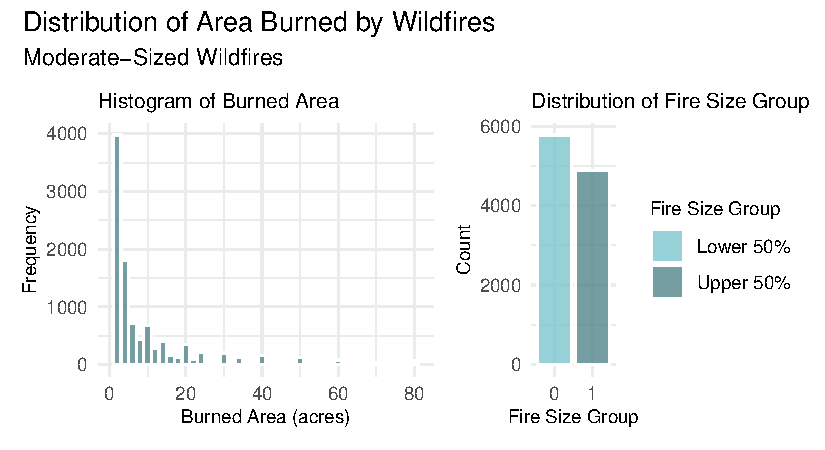
\includegraphics{written-report_files/figure-pdf/fire-size-dist-1.pdf}

Next, we visualized the distribution of the quantitative variables of
interest in our dataset (temperature (°C), relative humidity (\%), and
wind speed from 30 days prior to fire discovery (m/s), and remoteness).
We first examined the distribution of temperature a month before
discovery (top left panel), which we observed to be approximately normal
and unimodal. (This is consistent with what we would generally expect,
since temperature tends to change gradually across different areas
rather than clustering at specific values.) The median temperature for
wildfire observations in our dataset is 12.97 °C and the mean is 13.58
°C, with most observations between 6.53 °C and 21.36 °C. We then
examined the distributions of wind speed thirty days before discovery
and remoteness (top right and bottom left panels, respectively). Wind
speed appears to be very slightly right-skewed and unimodal, while
remoteness appears more strongly right-skewed and unimodal. This
indicates that most fires occurred relatively close to populated areas
(lower remoteness) and that most wind speeds were low to moderate. The
median remoteness for observations in our dataset is 0.21 and the mean
is 0.25, with most observations between 0.15 and 0.35. The median wind
speed for observations in our dataset is 2.89 m/s and the mean is 2.87
m/s, with most observations between 2.06 m/s and 3.76 m/s. Lastly, we
looked at the distribution of relative humidity thirty days before
discovery (bottom right panel), which appears to be left-skewed and
unimodal. This tells us that lower humidity conditions were more common
among wildfires in our data. The median relative humidity for
observations in our dataset is 63.53\% and the mean is 55.20\%, with
most observations between 48.80\% and 69.97\%. However, we noticed that
a large number of observations in our data recorded a relative humidity
of exactly 0\%. Given that 0\% relative humidity is unlikely under
normal atmospheric conditions (since even very dry air typically
contains some moisture), we decided to exclude these observations from
our analysis.

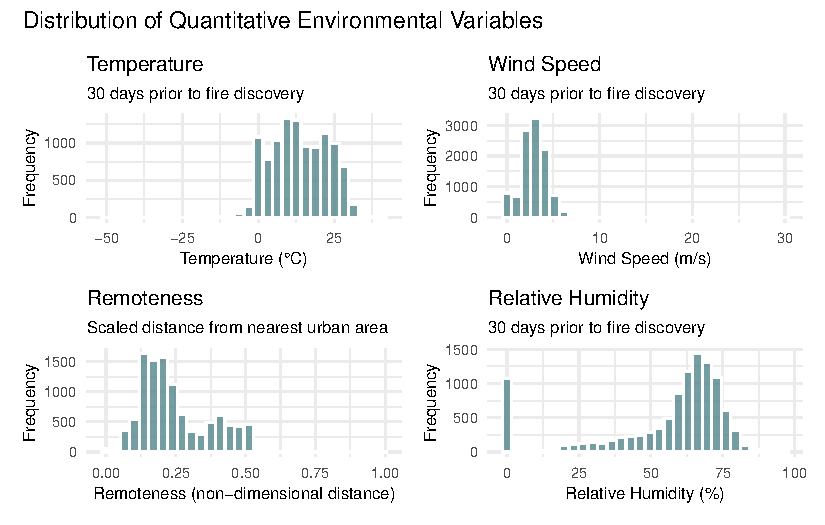
\includegraphics{written-report_files/figure-pdf/quantitative-univariate-eda-1.pdf}

In addition to examining the distributions of quantitative predictors,
we also visualized the distribution of categorical variables of interest
in our dataset (i.e., wildfire cause category, vegetation group, region,
and precipitation 30 days prior to wildfire discovery), which can be
found in the Appendix.

\FloatBarrier

\paragraph{Bivariate EDA}\label{bivariate-eda}

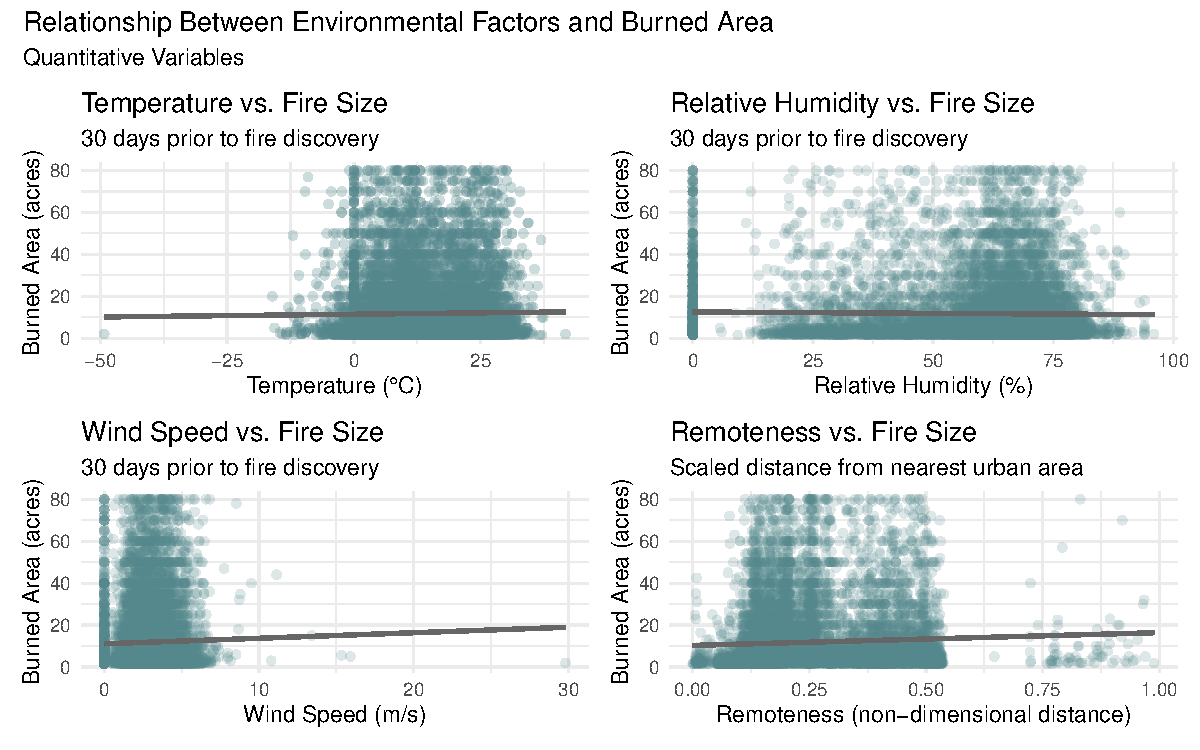
\includegraphics[width=0.9\textwidth,height=\textheight]{written-report_files/figure-pdf/fire-size-bivariate-1.pdf}

As the next step in our analysis, we examined the relationship between
each of our quantitative predictors and fire size to better understand
their associations. In the scatterplot of burned area versus temperature
(top left panel), the relationship appears very weak and slightly
positive (i.e., larger fires may be slightly more likely at higher
temperatures), but nonlinear, since most fires were small across the
temperature range, and the largest fires (over 60 acres) tended to occur
between 5 °C and 20 °C. The scatterplot of relative humidity versus
burned area (top right panel) also shows a very weak, highly nonlinear,
and slightly negative relationship, with fires of all sizes occurring
across the full humidity range and the largest fires more common between
25\% and 75\% humidity. For wind speed (bottom left panel), the
relationship appears very weak, slightly positive, and nonlinear; most
fires occurred at lower wind speeds, and most larger fires (over 40
acres) were concentrated below 5 m/s, suggesting that higher wind speeds
were not consistently associated with larger burned areas. In the
scatterplot of remoteness versus burned area (bottom right panel), we
observe a weak, slightly positive, and nonlinear relationship, with the
largest fires occurring between remoteness values of 0.25 and 0.50 and
relatively few large fires at very high remoteness values above 0.75.
Overall, the wide vertical spread of data points around the lines of
best fit for all predictors suggests that these quantitative predictors
have limited predictive power for burned area when considered
individually, which is expected given that wildfire size is influenced
by many factors beyond the variables available in our dataset.

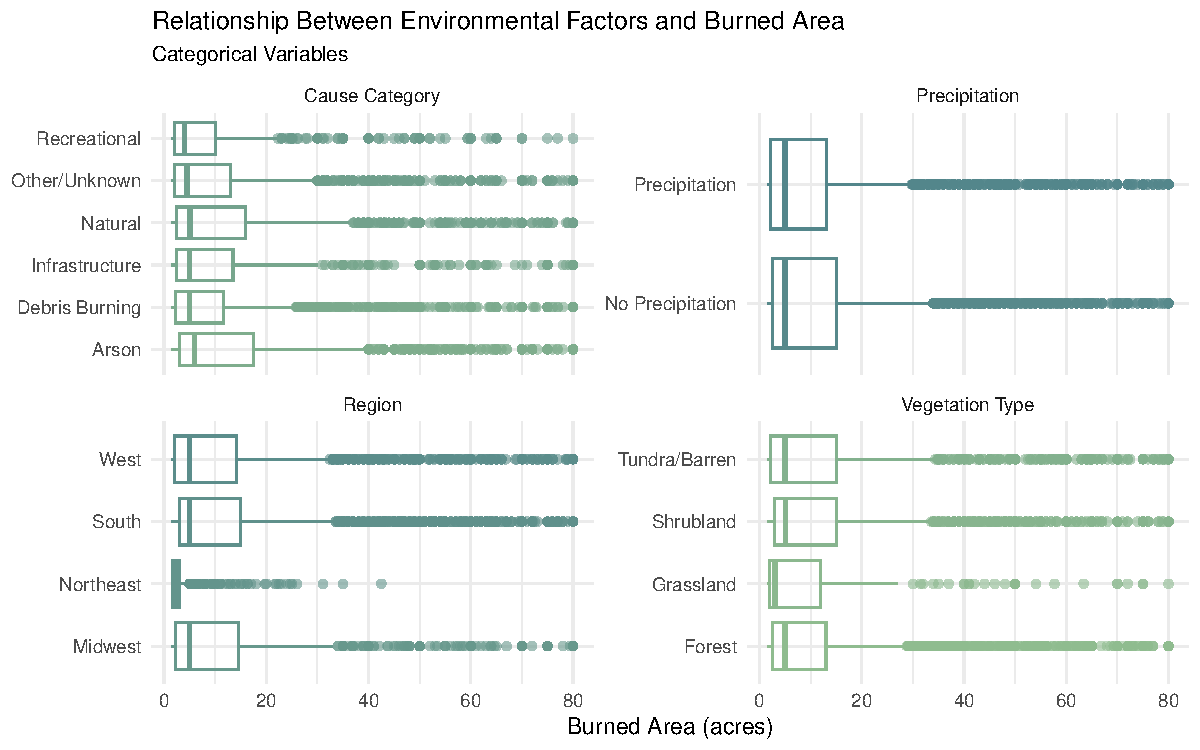
\includegraphics{written-report_files/figure-pdf/categorical-bivariate-dist-1.pdf}

As part of our bivariate EDA, we also analyzed the relationship between
each of our categorical variables of interest and burned area to better
understand differences in fire size across groups. We can see from the
visualization (top left panel) that the distribution of acres burned is
relatively similar for all wildfire cause categories, with medians
between 4.00 and 6.00 acres, means between 9.02 and 13.74 acres, and
outliers beyond the 30-acre mark across all cause types. This indicates
that cause category on its own does not explain much variability in fire
size. We observed a similar pattern between observations corresponding
to no precipitation 30 days before discovery and observations
corresponding to precipitation (top right panel), with both groups
showing medians of 5.00 acres and means of 12.32 acres (no
precipitation) and 11.38 acres (precipitation), although there was
slightly more spread in the middle 50\% of fires with no precipitation.
We observed more apparent differences in the distribution of acres
burned across different regions and vegetation groups (bottom left and
bottom right panels, respectively). In particular, the Northeast had a
lower median (3.00 acres) and mean (6.04 acres) compared to other
regions, with much less variability in the middle 50\% of fires and most
outliers limited to about the 40-acre mark. In contrast, distributions
for the West, South, and Midwest were more similar, with medians between
5.00 and 6.00 acres, means between 12.00 and 13.00 acres, and many
outliers beyond the 30-acre mark. For vegetation type, distributions
were fairly similar across categories, although grasslands had a
slightly lower median (4.00 acres) and mean (8.43 acres) compared to
other vegetation groups, with somewhat fewer extreme outliers. Overall,
region and vegetation group seem to explain more variability in fire
size compared to cause category or precipitation, and could be useful
predictors in modeling fire size.

\paragraph{Potential Interaction
Effects}\label{potential-interaction-effects}

Since many of our variables of interest relate to environmental
conditions and geographic location, there are potential interaction
effects among our predictors that could influence acres burned. As part
of our analysis, we were interested in a potential interaction between
vegetation type and precipitation, since vegetation and fuel moisture
could influence burned area together. Through our EDA, we observed that
acres burned did not seem to vary much across different precipitation
groups within each vegetation type. (A more detailed analysis of this
pattern is provided in the Appendix.)

\subsection{Methodology}\label{methodology}

The main goal of our analysis was to examine how various
wildfire-related factors are related to burned area, and how these
factors can be used to predict fire size. Since these represent two
distinct research questions, we chose to fit two separate models: a
linear regression model using all variables of interest (including those
only available after a fire is contained) to explain variability in
burned area (i.e., an explanatory model), and a logistic regression
model using only variables that are available at or before fire
discovery to guide response efforts to predict whether a wildfire burns
a greater-than-typical area (i.e., a predictive model). It is important
to note that our response variable, fire size, is continuous and
therefore suitable for linear regression. However, logistic regression
requires a binary response variable. (In this setup, the model estimates
the likelihood that a wildfire falls into the upper half of
moderate-sized fires based on available environmental factors.)

\paragraph{Multiple Linear Regression}\label{multiple-linear-regression}

To guide predictor selection for the explanatory model, we used a
forward selection approach based on adjusted \(R^2\) (which accounts for
model fit while penalizing unnecessary predictors), ultimately including
all predictors of interest (each contributed to an increase in adjusted
\(R^2\)). Our initial multiple linear regression predicted burned area
based on region, cause category, remoteness, vegetation group,
temperature, precipitation, wind speed, relative humidity (15 days
before discovery), containment time, and an interaction between
vegetation group and precipitation. We mean-centered the quantitative
predictors to improve coefficient interpretability. After fitting this
model, we conducted diagnostics to assess linearity, normality, constant
variance, and independence. Normality, linearity, and independence
appeared reasonably satisfied, but constant variance was violated, and
there was some evidence of potential non-linearity. To address constant
variance, we applied a variance-stabilizing (logarithmic) transformation
to the fire size variable. For linearity, we examined residuals against
each predictor and found no clear nonlinear patterns, so we did not
transform the predictors. When examining residuals versus fitted values,
we observed two distinct clusters (one with fitted values ≤5 and another
between 5 and 20), partly explained by differences across region
(specifically, smaller fires in the Northeast). We explored fitting
separate models for the Northeast and other regions but ultimately
proceeded with a single model because the improvement in fit was
minimal. We also checked for influential points using Cook's Distance
(\(D_i > 0.5\)) and found none. Lastly, we found collinearity between
levels corresponding to the Southern and Western regions; to address
this, we combined these levels into a single group, which helped reduce
collinearity without compromising interpretability. A detailed
assessment of model diagnostics (including residual plots, VIFs, and
checks for constant variance, linearity, and influential points) can be
found in the Appendix.

\paragraph{Logistic Regression}\label{logistic-regression}

To guide variable selection for the predictive model, we fit a full
model including all variables of interest. This approach was appropriate
because our dataset contained a limited number of predictors
corresponding to information available prior to fire discovery, making
it practical to include all relevant variables rather than selecting a
smaller subset. Specifically, our initial logistic regression model
predicted the likelihood that a wildfire would burn a
greater-than-typical area based on temperature, humidity, wind speed,
precipitation, vegetation type, the interaction between vegetation type
and precipitation, remoteness, and region. After fitting the model, we
determined that the key assumptions for logistic regression (linearity,
randomness, and independence) were satisfied. A detailed assessment of
model diagnostics (empirical logit plots, assessment of logistic
regression conditions) can be found in the Appendix.

\subsection{Results}\label{results}

\paragraph{Multiple Linear
Regression}\label{multiple-linear-regression-1}

\begin{table}[!h]
\centering\begingroup\fontsize{7}{9}\selectfont

\begin{tabular}{lrrrrrr}
\toprule
term & estimate & std.error & statistic & p.value & conf.low & conf.high\\
\midrule
(Intercept) & 1.997 & 0.045 & 44.329 & 0.000 & 1.909 & 2.085\\
regionNortheast & -0.942 & 0.059 & -16.003 & 0.000 & -1.057 & -0.826\\
regionSouth\_West & 0.075 & 0.036 & 2.072 & 0.038 & 0.004 & 0.145\\
cause\_categoryDebris Burning & -0.255 & 0.029 & -8.676 & 0.000 & -0.313 & -0.198\\
cause\_categoryInfrastructure & -0.113 & 0.043 & -2.630 & 0.009 & -0.198 & -0.029\\
\addlinespace
cause\_categoryNatural & -0.050 & 0.038 & -1.308 & 0.191 & -0.125 & 0.025\\
cause\_categoryOther/Unknown & -0.160 & 0.032 & -5.014 & 0.000 & -0.222 & -0.097\\
cause\_categoryRecreational & -0.370 & 0.042 & -8.701 & 0.000 & -0.453 & -0.286\\
remoteness & -0.310 & 0.099 & -3.118 & 0.002 & -0.504 & -0.115\\
Vegetation\_groupGrassland & 0.189 & 0.089 & 2.130 & 0.033 & 0.015 & 0.362\\
\addlinespace
Vegetation\_groupShrubland & 0.065 & 0.027 & 2.432 & 0.015 & 0.013 & 0.118\\
Vegetation\_groupTundra/Barren & 0.073 & 0.026 & 2.767 & 0.006 & 0.021 & 0.125\\
Prec\_pre\_15\_cent & 0.025 & 0.031 & 0.793 & 0.428 & -0.036 & 0.086\\
Wind\_pre\_15\_cent & 0.032 & 0.008 & 3.929 & 0.000 & 0.016 & 0.047\\
Temp\_pre\_15\_cent & -0.003 & 0.001 & -2.643 & 0.008 & -0.006 & -0.001\\
\addlinespace
Hum\_pre\_15\_cent & -0.001 & 0.001 & -1.131 & 0.258 & -0.002 & 0.000\\
putout\_time\_num & 0.007 & 0.001 & 5.183 & 0.000 & 0.004 & 0.010\\
Vegetation\_groupGrassland:Prec\_pre\_15\_cent & -0.203 & 0.168 & -1.206 & 0.228 & -0.532 & 0.127\\
Vegetation\_groupShrubland:Prec\_pre\_15\_cent & -0.141 & 0.051 & -2.770 & 0.006 & -0.241 & -0.041\\
Vegetation\_groupTundra/Barren:Prec\_pre\_15\_cent & 0.018 & 0.051 & 0.349 & 0.727 & -0.082 & 0.118\\
\bottomrule
\end{tabular}
\endgroup{}
\end{table}

Our final multiple linear regression model predicting log-transformed
fire size achieved an \(R^{2}\) of 0.052 and an adjusted \(R^2\) of
0.050 (model results in Appendix). This indicates that the model
explains approximately 5.0\% of the variability in log-transformed
burned area among moderate-sized wildfires in the dataset. While low,
this amount of explained variance is expected given the variability in
wildfire behavior and the limited set of predictors available. We
examined several predictors in our model and found that region, cause
category, remoteness, vegetation group, wind speed 15 days prior to
discovery, temperature 15 days prior to discovery, putout time, and the
interaction between shrubland vegetation and precipitation were
significant predictors of log-transformed fire size (p \textless{}
0.05). In contrast, relative humidity 15 days prior (p \textgreater{}
0.05), precipitation 15 days prior (p \textgreater{} 0.05), and the
interaction terms between grassland or tundra/barren vegetation and
precipitation (p \textgreater{} 0.05) were not significant; this result
is consistent with our EDA findings (i.e., differences across region and
vegetation type and the effect of wind speed were more apparent, while
precipitation and humidity did not show strong relationships with fire
size). The intercept of the model is estimated at 2.000, indicating that
the expected fire size is approximately \(e^{2.000} \approx 7.39\) acres
when all predictors are at their reference or mean-centered values
(i.e., for a wildfire in the Midwest region, caused by arson, in a
forested area, under average environmental conditions --- mean
temperature = 13.8°C, mean relative humidity = 52.0\%, mean wind speed =
2.77 m/s, mean remoteness = 0.252 --- and with putout time equal to 0).
Fires caused by recreational activities are expected to burn about
\(e^{-0.370} \approx 0.69\) times the acres compared to fires caused by
arson, holding other factors constant. Fires caused by debris burning
are expected to burn approximately \(e^{-0.255} \approx 0.78\) times the
acres compared to arson-related fires. Additionally, fires occurring in
the Northeast are expected to burn about \(e^{-0.942} \approx 0.39\)
times the acres relative to fires in the Midwest. Other predictors,
including vegetation group, environmental conditions (such as wind speed
and temperature), remoteness, containment time, and
vegetation--precipitation interactions, also showed statistically
significant associations with fire size, although their effects were
generally smaller in magnitude.

\paragraph{Logistic Regression}\label{logistic-regression-1}

\begin{table}[!h]
\centering\begingroup\fontsize{7}{9}\selectfont

\begin{tabular}{lrrrrrr}
\toprule
term & estimate & std.error & statistic & p.value & conf.low & conf.high\\
\midrule
(Intercept) & -0.220 & 0.098 & -2.257 & 0.024 & -0.412 & -0.029\\
regionNortheast & -1.829 & 0.148 & -12.363 & 0.000 & -2.125 & -1.545\\
regionSouth\_West & 0.182 & 0.069 & 2.642 & 0.008 & 0.047 & 0.316\\
remoteness & -0.414 & 0.182 & -2.271 & 0.023 & -0.772 & -0.057\\
Vegetation\_groupGrassland & 0.635 & 0.273 & 2.328 & 0.020 & 0.104 & 1.179\\
\addlinespace
Vegetation\_groupShrubland & 0.209 & 0.064 & 3.246 & 0.001 & 0.083 & 0.335\\
Vegetation\_groupTundra/Barren & 0.093 & 0.069 & 1.344 & 0.179 & -0.043 & 0.228\\
Prec\_pre\_15 & 0.032 & 0.060 & 0.533 & 0.594 & -0.086 & 0.150\\
Wind\_pre\_15 & 0.036 & 0.016 & 2.291 & 0.022 & 0.005 & 0.066\\
Temp\_pre\_15 & -0.005 & 0.002 & -1.988 & 0.047 & -0.009 & 0.000\\
\addlinespace
Hum\_pre\_15 & -0.001 & 0.001 & -0.632 & 0.527 & -0.003 & 0.001\\
Vegetation\_groupGrassland:Prec\_pre\_15 & -0.641 & 0.347 & -1.849 & 0.064 & -1.328 & 0.034\\
Vegetation\_groupShrubland:Prec\_pre\_15 & -0.185 & 0.097 & -1.897 & 0.058 & -0.375 & 0.006\\
Vegetation\_groupTundra/Barren:Prec\_pre\_15 & 0.012 & 0.099 & 0.121 & 0.904 & -0.182 & 0.206\\
\bottomrule
\end{tabular}
\endgroup{}
\end{table}

Our final logistic regression model predicting whether a wildfire burns
a greater-than-typical area achieved an AUC of 0.569, indicating a
relatively limited ability to distinguish between smaller and larger
moderate-sized fires based on the predictors included (AUC value and
corresponding ROC curve are provided in the Appendix). After fitting the
full model with an interaction between vegetation group and
precipitation, we conducted a drop-in-deviance test to assess whether
the interaction terms were jointly useful. Since the p-value for the
test was 0.013, we retained the interaction between vegetation group and
precipitation (full test results are provided in the Appendix); while
the individual interaction terms were not significant at the 0.05 level,
the combined contribution significantly improved model fit. We examined
several predictors in our model and found that region, remoteness,
vegetation group (grassland and shrubland), wind speed 15 days prior,
and temperature 15 days prior were significant predictors of fire size
classification (p \textless{} 0.05). In contrast, relative humidity 15
days prior (p \textgreater{} 0.05), precipitation 15 days prior (p
\textgreater{} 0.05), tundra/barren vegetation group (p \textgreater{}
0.05), and the interaction terms between vegetation group and
precipitation (p \textgreater{} 0.05) were not significant. The
intercept of the model is estimated at -0.220, which indicates that the
expected odds of a wildfire falling into the larger half of
moderate-sized fire sizes is approximately \(e^{-0.220} \approx 0.80\)
when all predictors are at their reference or mean-centered values
(i.e., for a wildfire in the Midwest region, in a forested area, with no
precipitation 15 days prior, and under average environmental conditions
--- mean temperature = 13.8°C, mean relative humidity = 52.0\%, mean
wind speed = 2.77 m/s, mean remoteness = 0.252). Fires in the Northeast
are expected to have approximately \(e^{-1.830} \approx 0.16\) times the
odds of falling into the upper 50\% compared to fires in the Midwest,
holding all else constant. Fires occurring in shrublands are associated
with approximately \(e^{0.209} \approx 1.23\) times the odds compared to
fires occurring in forests, controlling for other variables. Other
predictors such as remoteness, wind speed, and temperature also had
statistically significant effects on fire size classification, although
their individual impacts were smaller in magnitude.

\subsection{Discussion and Conclusion}\label{discussion-and-conclusion}

Our analysis used both multiple linear regression and logistic
regression to understand factors associated with wildfire size in the
United States. The multiple linear regression model, which predicted
log-transformed fire size, found that physical factors like vegetation
type, wind speed, precipitation, temperature, and humidity and other
factors including region, remoteness, fire cause, and containment time
were significant predictors, though the model explained only about 5\%
of the variability in fire size. The logistic regression model, which
predicted the likelihood that a wildfire burned a greater-than-typical
area, used similar predictors except the cause of the fire, but did not
have a very effective classification ability (AUC = 0.569). In both
models, fires in shrubland and grassland were associated with larger
burned areas, while fires in the Northeast tended to be smaller. Greater
wind speeds slightly increased fire size, and greater remoteness was
associated with smaller fires.

There were several limitations to our analysis. While the number of
fires in the dataset was massive, comprehensive data on those fires was
often limited, which likely contributed to the low explanatory power of
our models. Because the data spanned more than two decades, changes over
time in climate patterns, land use, and fire management practices could
have introduced variability that our models did not account for.
Although most model assumptions were satisfied after transformations,
there were issues with non- variance that could affect the reliability
of our conclusions.

Future work could focus a lot on improving data by collecting more data
points for each of the fires. While technology can be limited in this
aspect, especially for fires that may be in remote regions, better
quality data could be very effective in helping to understand where
resources need to go to put out fires and solve this important problem.
Despite these limitations, our models did uncover some important factors
of wildfire size and confirmed the need for more detailed data to
support effective wildfire prediction and management.

\newpage

\subsection{Appendix}\label{appendix}

\paragraph{Exploratory Data Analysis - Bivariate EDA for Categorical
Predictors}\label{exploratory-data-analysis---bivariate-eda-for-categorical-predictors}

Looking more closely at vegetation group, we can see that most fires
occurred in forested areas (5181 observations or 48.6\%), followed by
shrubland (2711 observations or 25.4\%) and tundra or barren areas (2590
observations or 24.3\%), with relatively few fires in grassland
environments (189 observations or 1.77\%). Examining wildfire cause
categories, we found that a large portion of fires were attributed to
human-related causes rather than natural causes. Debris burning
accounted for the highest proportion (2821 observations or 26.4\%),
followed by arson (2399 observations or 22.5\%) and other or unknown
causes (2228 observations or 20.9\%). Natural causes made up a smaller
proportion (1535 observations or 14.4\%), followed by recreational
causes (853 observations or 8.0\%) and infrastructure-related causes
(835 observations or 7.82\%). Finally, we examined the regional
distribution of fires. Most fires in our dataset occurred in the South
(6090 observations or 57.1\%), followed by the West (2801 observations
or 26.2\%), Midwest (1228 observations or 11.5\%), and Northeast (550
observations or 5.15\%). Only two fires (2 observations or less than
0.01\%) were categorized as occurring in the ``Other'' region
classification.

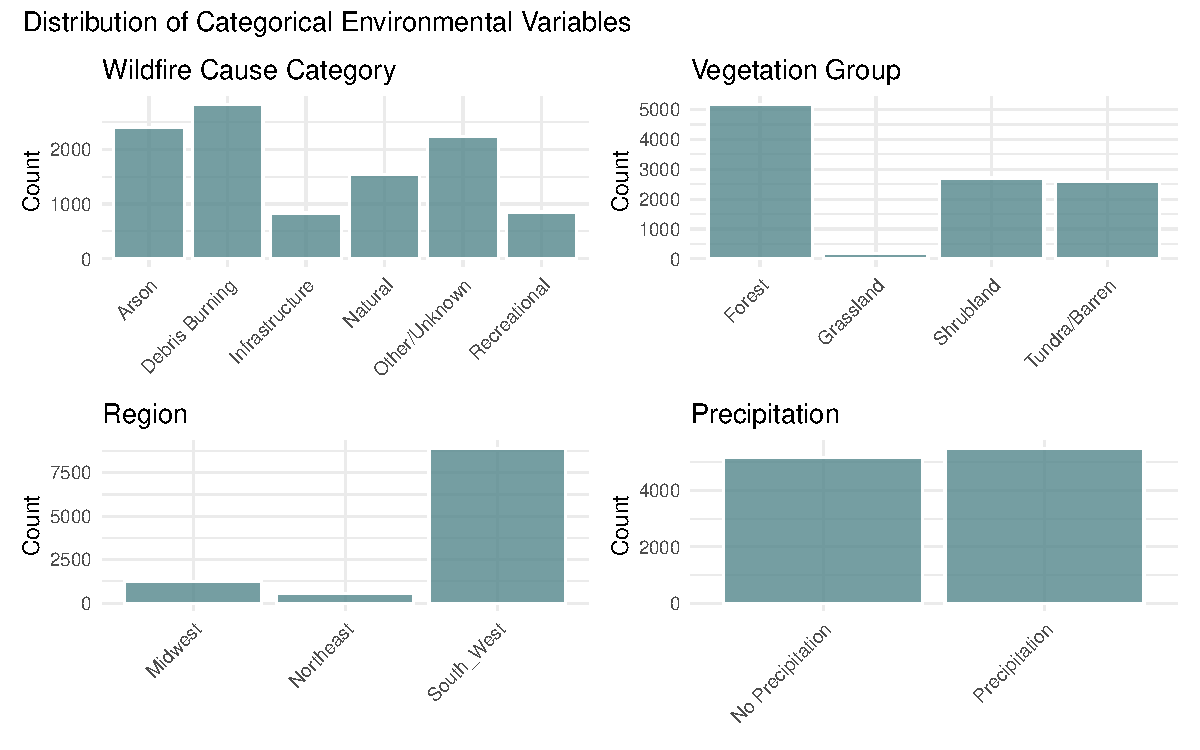
\includegraphics{written-report_files/figure-pdf/categorical-dist-1.pdf}

\paragraph{Exploratory Data Analysis - Potential Interaction
Effects}\label{exploratory-data-analysis---potential-interaction-effects}

In our analysis, we were interested in a potential interaction between
vegetation type and precipitation. Based on the visualization below, the
distributions of burned area appearrelatively similar between
precipitation and no precipitation conditions for each vegetationgroup.
In forest, the median burned area is 5.0 acres for both no precipitation
(mean of 11.48acres) and precipitation (mean of 11.14 acres), while in
grassland, the median is 3.5 acresfor no precipitation (mean 12.26
acres) and 3.0 acres for precipitation (mean of 11.54
acres).Additionally, in shrubland, the median is 6.0 acres for no
precipitation (mean of 13.52 acres)and 5.0 acres for precipitation (mean
of 11.31 acres), while in tundra/barren, the median is 5.0 acres for
both no precipitation (mean of 12.81 acres) and precipitation (mean of
11.86 acres).Even though there does not appear to be a very strong
effect, this interaction would be worthexploring more formally in the
modeling process to determine whether it significantly improvesmodel
fit.

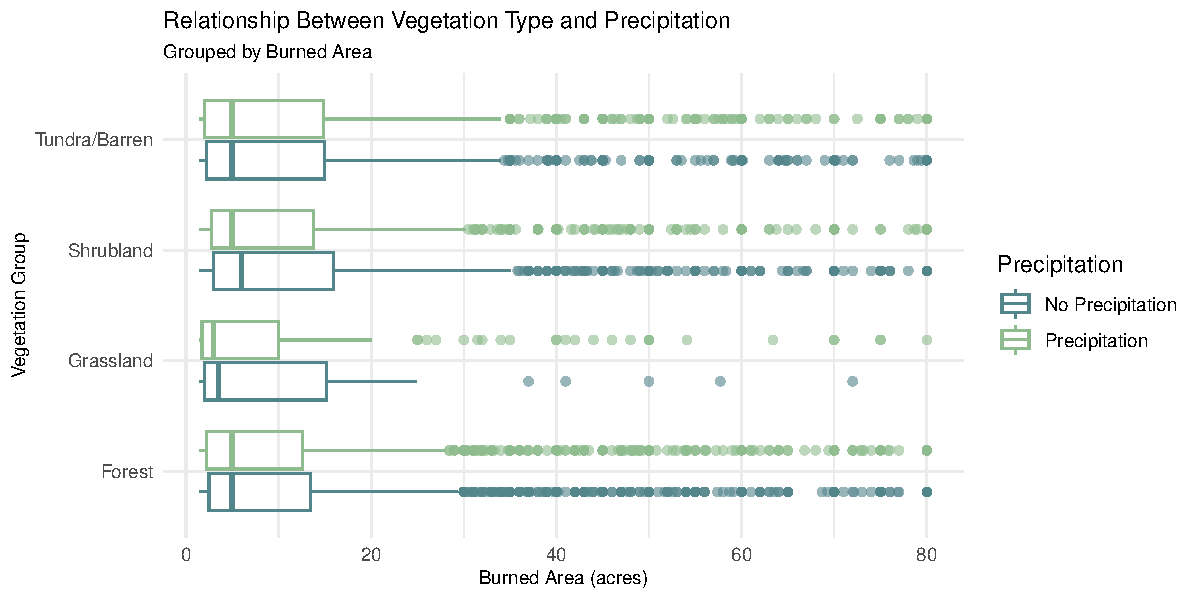
\includegraphics{written-report_files/figure-pdf/veg-prec-int-1.pdf}

\paragraph{Methods - Explanatory
Model}\label{methods---explanatory-model}

A scatterplot of residuals vs.~fitted values for our explanatory model
is shown below. Given that the initial model we fit had a clear
violation of constant variance (an increase in the variability of
residuals as fitted values increased), we applied a variance-stabilizing
(i.e., logarithmic) transformation to the response variable. We observed
an improvement in the spread of residuals (more uniform spread across
the range of fitted values) as well as a slight improvement in model fit
(an increase in adjusted \(R^2\)) after applying this transformation.
Because there was also a clear pattern in the residuals (i.e., they were
not randomly scattered around \(residuals = 0\)), we examined
scatterplots of fitted values versus each of the predictors and observed
no clear nonlinear trends. As a result, we did not transform our
predictors. We also did not observe any influential points
(\(D_i > 0.5\)) in our data, so no observations were removed. Lastly, we
observed two distinct groupings in the scatterplot of residuals
vs.~fitted values (one group with fitted values less than 1.5 and one
group with fitted values generally above 1.5). We found that a large
portion of this separation could be explained by region, so we fit
separate linear regression models for different regional groups.
However, this approach did not lead to a meaningful increase in
explanatory power, so we retained a single model for all observations.
From our work, we deem that constant variance and linearity are
sufficiently satisfied.

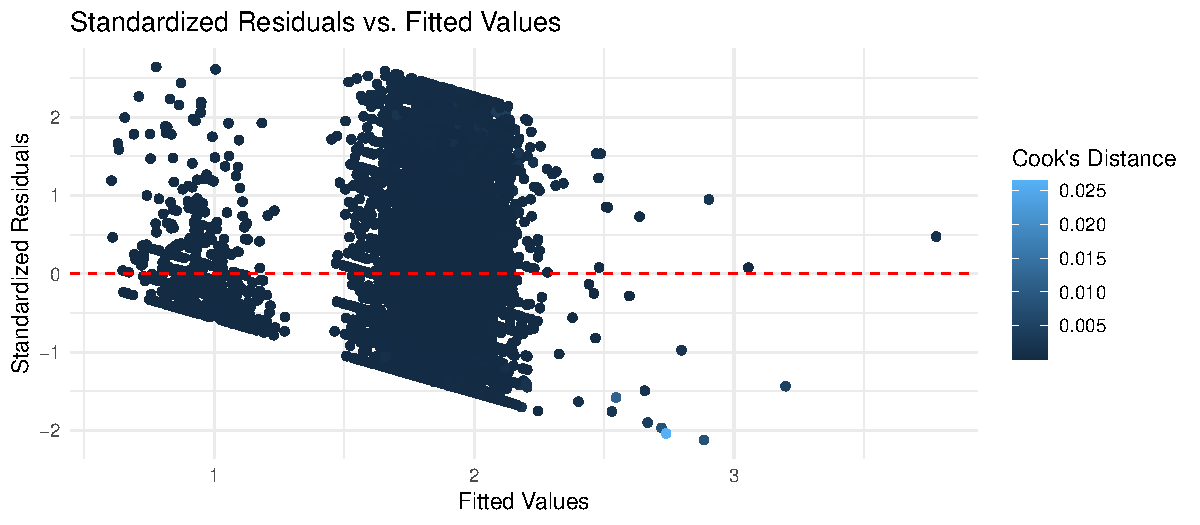
\includegraphics{written-report_files/figure-pdf/residuals-fitted-vals-plot-1.pdf}

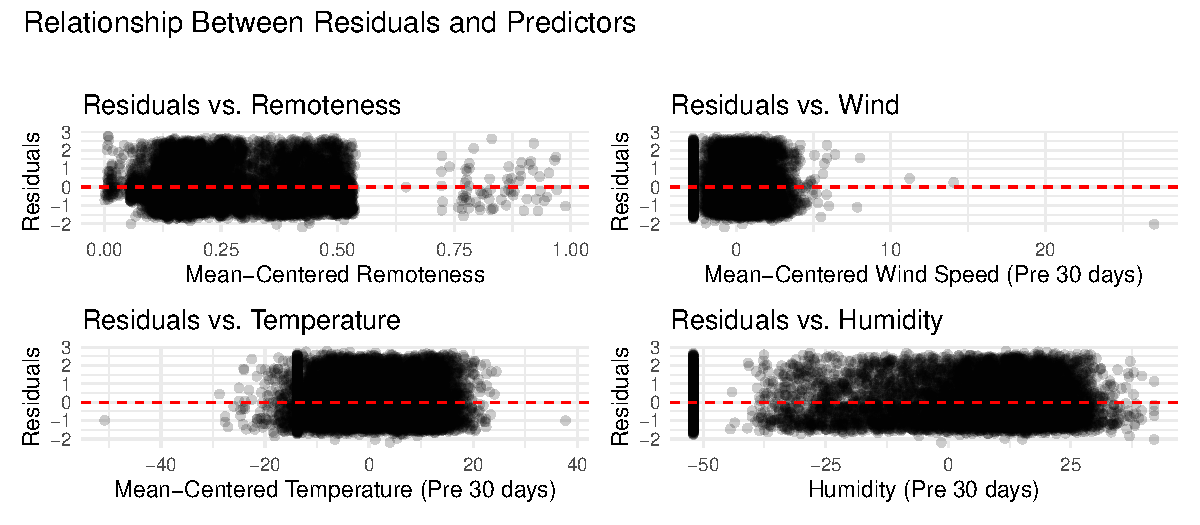
\includegraphics{written-report_files/figure-pdf/residuals-fitted-vals-plot-2.pdf}

While the distribution of residuals is skewed right, we have far more
than 30 observation, so we can assume normality is satisfied.

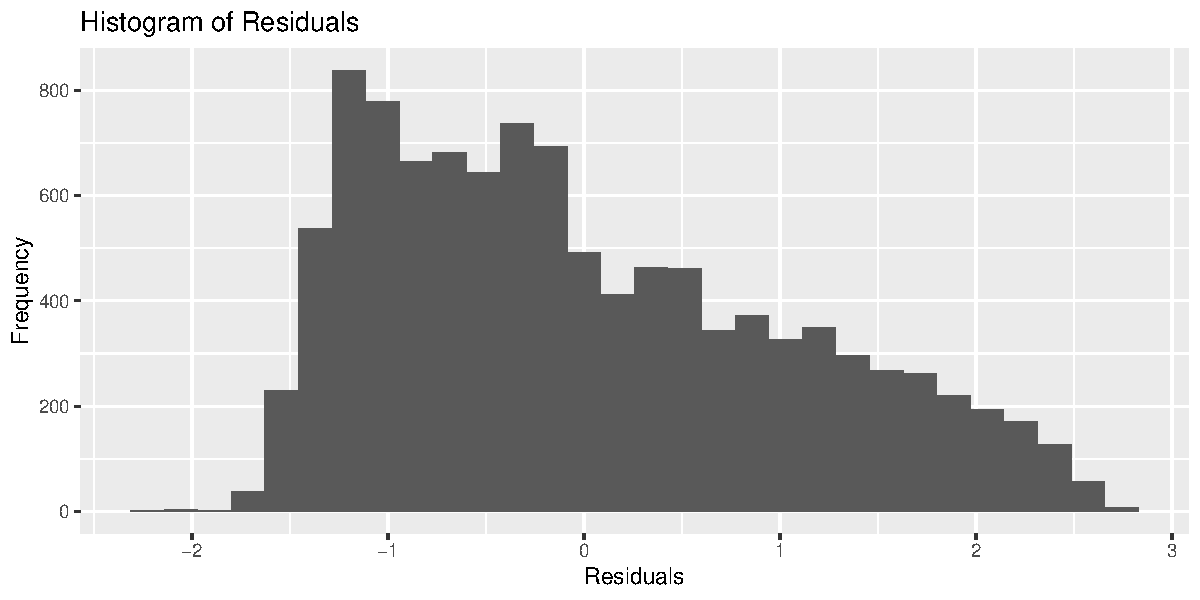
\includegraphics{written-report_files/figure-pdf/unnamed-chunk-12-1.pdf}

We also screened for potential collinearity between our predictors and,
while we initially observed some concerning multicollinearity between
levels of our region variable (\(VIF > 5\)), we addressed this by
collapsing the South and West levels of the variable together and
refitting the model based on the recoded version. All of the VIFs for
the updated model are less than 5, indicating no issues with
multicollinearity among the predictors.

\begingroup\fontsize{7}{9}\selectfont

\begin{longtable*}[t]{cc}
\toprule
Predictor & VIF\\
\midrule
Prec\_pre\_15\_cent & 2.29\\
cause\_categoryNatural & 1.74\\
regionSouth\_West & 1.74\\
remoteness & 1.69\\
regionNortheast & 1.63\\
\addlinespace
cause\_categoryDebris Burning & 1.62\\
cause\_categoryOther/Unknown & 1.62\\
Hum\_pre\_15\_cent & 1.58\\
Vegetation\_groupTundra/Barren:Prec\_pre\_15\_cent & 1.54\\
Vegetation\_groupShrubland:Prec\_pre\_15\_cent & 1.53\\
\addlinespace
Wind\_pre\_15\_cent & 1.42\\
Temp\_pre\_15\_cent & 1.38\\
Vegetation\_groupShrubland & 1.31\\
Vegetation\_groupGrassland & 1.31\\
Vegetation\_groupGrassland:Prec\_pre\_15\_cent & 1.31\\
\addlinespace
cause\_categoryInfrastructure & 1.29\\
cause\_categoryRecreational & 1.28\\
Vegetation\_groupTundra/Barren & 1.23\\
putout\_time\_num & 1.04\\
\bottomrule
\end{longtable*}
\endgroup{}

Lastly, we looked for any spatial and temporal correlations in residuals
and found no apparent patterns, so independence can be considered
reasonably satisfied.

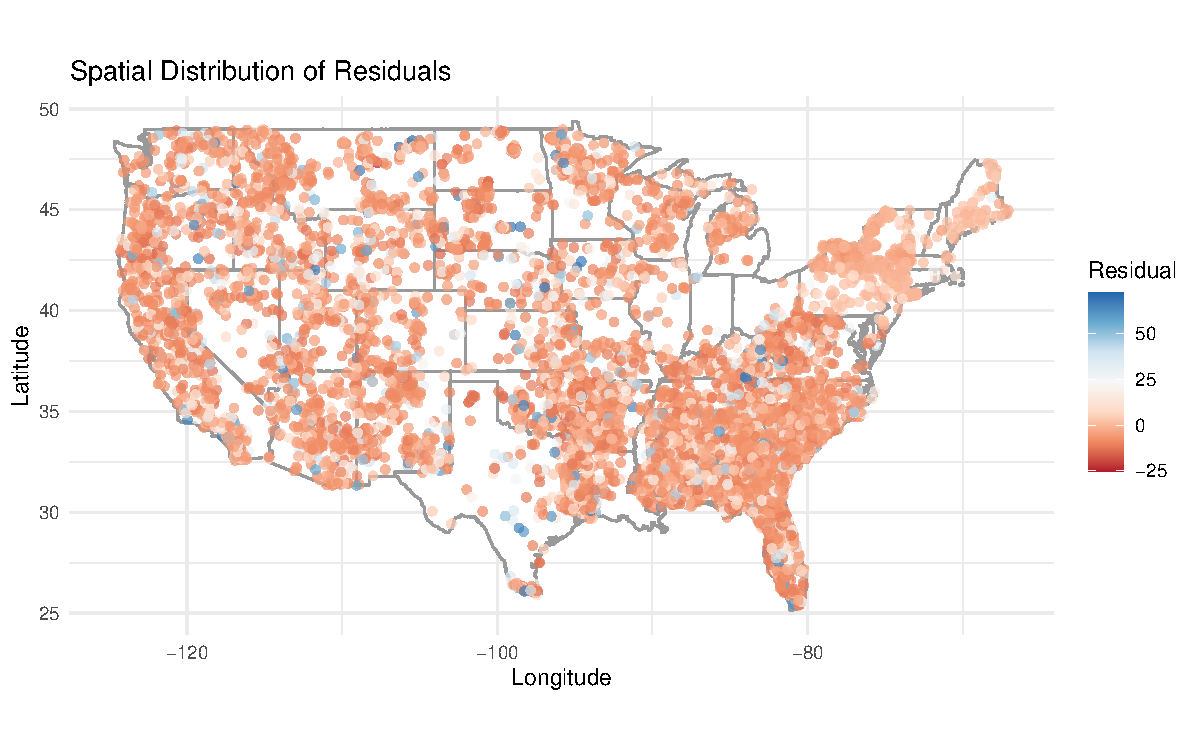
\includegraphics{written-report_files/figure-pdf/spatial-distribution-residuals-1.pdf}

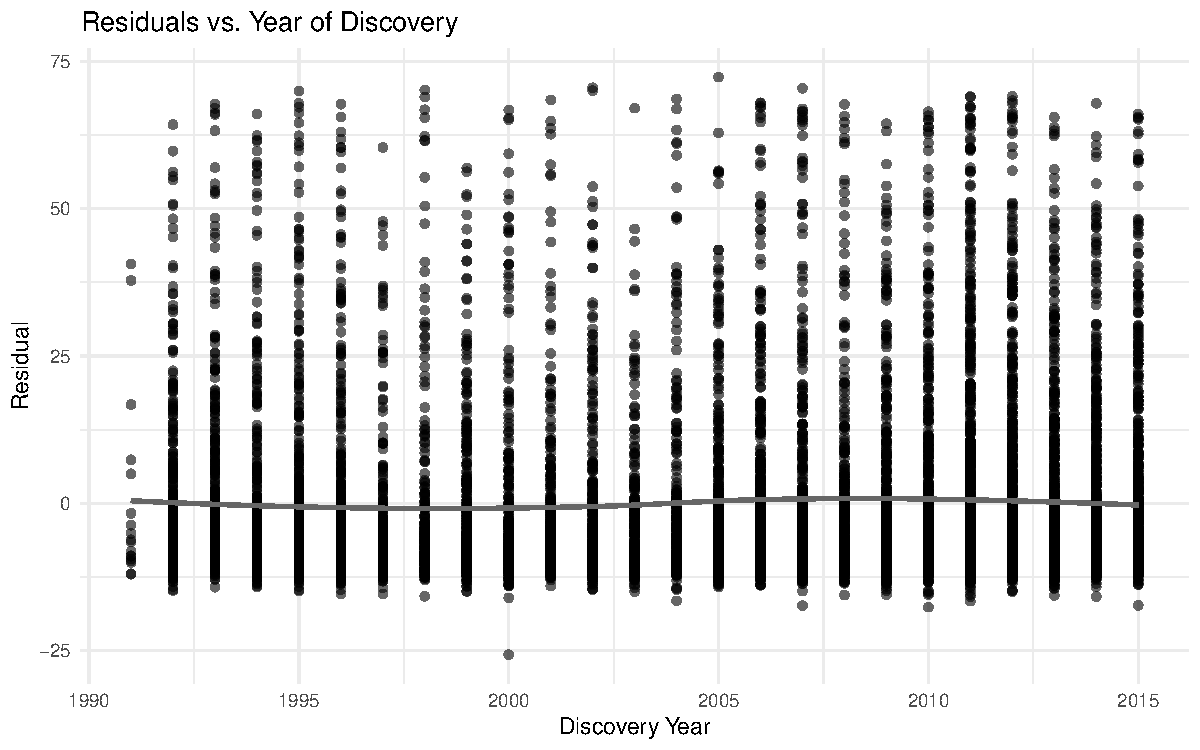
\includegraphics{written-report_files/figure-pdf/spatial-distribution-residuals-2.pdf}

\paragraph{Methods - Predictive Model}\label{methods---predictive-model}

Wildfire records in our dataset can reasonably be treated as independent
because, in our assessment of the independence condition for linear
regression, we observed no spatial correlations between residuals and
geographic location. The randomness assumption was satisfied because the
wildfire data were compiled from a large national database covering a
wide range of fires across the United States between 1992 and 2015,
making it reasonable to assume the dataset is representative of the
broader wildfire population. Lastly, the linearity condition appears to
be reasonably satisfied, as empirical logit plots for the quantitative
predictors did not display strong deviations from linearity, and the
assumption of linearity in the log-odds was met.

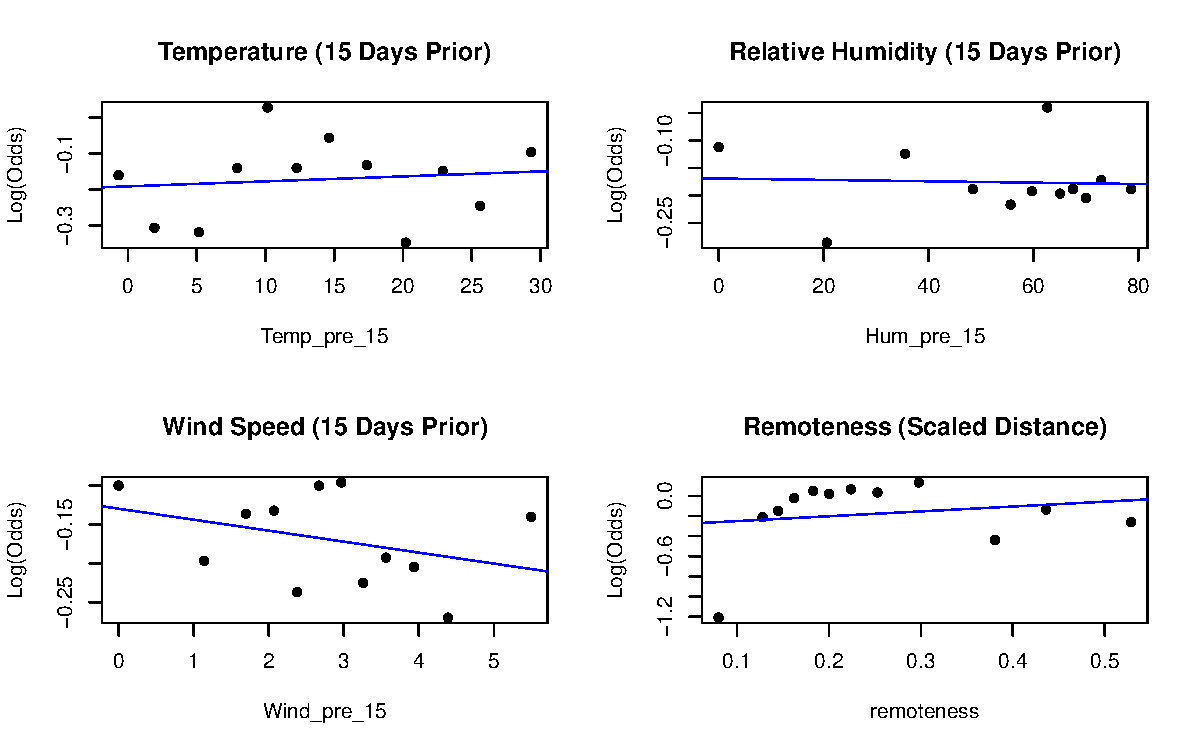
\includegraphics{written-report_files/figure-pdf/unnamed-chunk-15-1.pdf}

\paragraph{Results - Explanatory
Model}\label{results---explanatory-model}

The estimated multiple linear regression equation predicting
log-transformed fire size is shown below:

\[
\begin{aligned}
\widehat{\log(\text{Fire Size})} =\ &\ 2.00 \\
&- 0.94\,\cdot\,\text{Region (Northeast, South/West)} \\
&- 0.26\,\cdot\,\text{Cause Category (Debris, Infrastructure, Other/Unknown, Recreational)} \\
&- 0.31\,\cdot\,\text{Remoteness} \\
&+ 0.19\,\cdot\,\text{Vegetation Group (Grassland, Shrubland, Tundra/Barren)} \\
&+ 0.03\,\cdot\,\text{Wind Speed (15 days prior)} \\
&- 0.00\,\cdot\,\text{Temperature (15 days prior)} \\
&+ 0.01\,\cdot\,\text{Containment Time} \\
&- 0.14\,\cdot\,(\text{Vegetation Group} \times \text{Precipitation (15 days prior)})
\end{aligned}
\]

Additionally, \(R^2\) and adjusted \(R^2\) values for the fitted model
are displayed below:

\begin{table}[!h]
\centering\begingroup\fontsize{7}{9}\selectfont

\begin{tabular}{rr}
\toprule
R² & Adjusted R²\\
\midrule
0.052 & 0.05\\
\bottomrule
\end{tabular}
\endgroup{}
\end{table}

\paragraph{Results - Predictive Model}\label{results---predictive-model}

The estimated logistic regression equation predicting the log-odds that
a wildfire falls into the upper 50\% of moderate-sized fires is shown
below.

\[
\begin{aligned}
\log\left(\frac{\hat{\pi}}{1-\hat{\pi}}\right) =\ &\ -0.22 \\
&- 1.83\,\cdot\,\text{Northeast region} \\
&+ 0.18\,\cdot\,\text{South/West region} \\
&- 0.41\,\cdot\,\text{Remoteness} \\
&+ 0.64\,\cdot\,\text{Grassland vegetation} \\
&+ 0.21\,\cdot\,\text{Shrubland vegetation} \\
&+ 0.09\,\cdot\,\text{Tundra/Barren vegetation} \\
&+ 0.03\,\cdot\,\text{Precipitation (15 days prior)} \\
&+ 0.04\,\cdot\,\text{Wind speed (15 days prior)} \\
&- 0.00\,\cdot\,\text{Temperature (15 days prior)} \\
&- 0.00\,\cdot\,\text{Relative humidity (15 days prior)} \\
&- 0.64\,\cdot\,(\text{Grassland vegetation} \times \text{Precipitation}) \\
&- 0.19\,\cdot\,(\text{Shrubland vegetation} \times \text{Precipitation}) \\
&+ 0.01\,\cdot\,(\text{Tundra/Barren vegetation} \times \text{Precipitation})
\end{aligned}
\]

Additionally, the ROC curve for this model is presented below. We
observed an AUC of 0.569, indicating relatively limited discriminative
ability between fires falling into the upper 50\% of moderate-sized
fires and those falling into the lower 50\%. As we can see in the ROC
curve, as the true negative rate increases, sensitivity increases only
gradually, which indicates limited improvement in correctly identifying
larger fires (even as the true negative rate improves).

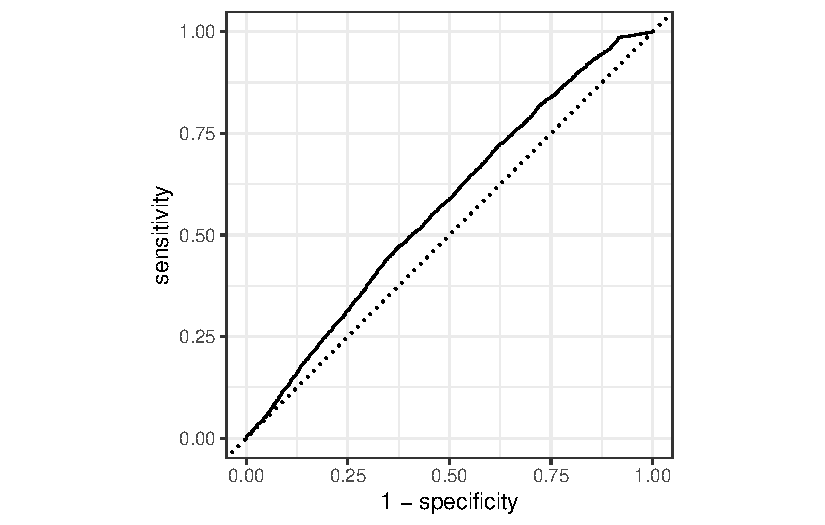
\includegraphics{written-report_files/figure-pdf/unnamed-chunk-17-1.pdf}

\begin{verbatim}
# A tibble: 1 x 3
  .metric .estimator .estimate
  <chr>   <chr>          <dbl>
1 roc_auc binary         0.569
\end{verbatim}

Lastly, the results of the drop-in-deviance test for our logistic
regression are presented below. Since the p-value (0.013) was less than
0.05, we retained the interaction between vegetation group and
precipitation in the model.

\begin{table}
\centering\begingroup\fontsize{7}{9}\selectfont

\begin{tabular}{cccccc}
\toprule
Model & Residual df & Residual Deviance & Test df & Test Deviance & p-value\\
\midrule
\makecell{mid50\_hi ~ region + remoteness + \\ Wind\_pre\_15 + Temp\_pre\_15 + Hum\_pre\_15} & 10662 & 14399.02 & NA & NA & NA\\
\makecell{mid50\_hi ~ region + remoteness + \\ Vegetation\_group * Prec\_pre\_15 + \\ Wind\_pre\_15 + Temp\_pre\_15 + Hum\_pre\_15} & 10655 & 14381.18 & 7 & 17.839 & 0.013\\
\bottomrule
\end{tabular}
\endgroup{}
\end{table}




\end{document}
